\newpage
\slidetitle{}
\section{Zusammenfassung und Ausblick \\}


\begin{itemize}
	\item Lindenmayer-Systeme\\
	
	\item Space Colonization Algorithmus\\
	
	\item Implementierung und Ergebnisse
\end{itemize}


\newpage
\slidetitle{6. Zusammenfassung - Bewertung}
\subsection{Bewertung der Ergebnisse - Visuell\\}

\paragraph{L-Systeme\\}

\begin{itemize}
	\item[$+$] Genaue Kontrolle über generierte Baumstrukturen\\
	
	\item[$+$] Unterschiedliche Strukturen bei gleichbleibender L-System Definition möglich\\
	
	\item[$-$] Muster und Regelmäßigkeiten sind erkennbar
\end{itemize}




\newpage
\paragraph{Space Colonization Algorithmus\\}

\begin{itemize}
	\item[$+$] Für die Darstellung von unregelmäßigen, komplexen Baumstrukturen geeignet\\
	
	\item[$+$] Generiert auch ohne Ergänzungen realistische Formen\\
	
	\item[$+$] Anpassung der Baumstruktur an einschränkende Bedingungen\\
	
	\item[$-$] Für die Darstellung vieler Baumsorten nicht geeignet\\
\end{itemize}




\newpage
\subsection{Bewertung der Ergebnisse - Effizienz\\}

\paragraph{L-Systeme\\}

\begin{itemize}
	\item[$+$] Vergleichsweise schnelle Generierung\\
	
	\item[$-$] Benötigt eine vergleichsweise große Menge Modelldaten für die Darstellung realistisch wirkender Strukturen\\
	
	\item[$-$] Menge der Modelldaten nur durch L-System Definition beeinflussbar
\end{itemize}





\newpage
\paragraph{Space Colonization Algorithmus\\}

\begin{itemize}
	\item[$+$] Generierte Datenmenge lässt sich durch Algorithmus-Parameter und Kurvenreduktion anpassen\\
	
	\item[$+$] Verringerung der Datenmenge ohne visuelle Beeinträchtigung möglich\\
	
	\item[$-$] Vergleichsweise lange Generierungszeit\\
	
	\item[$\pm$] Generierungszeit stark von bestimmten Parametern abhängig
\end{itemize}




\newpage
\begin{center}
	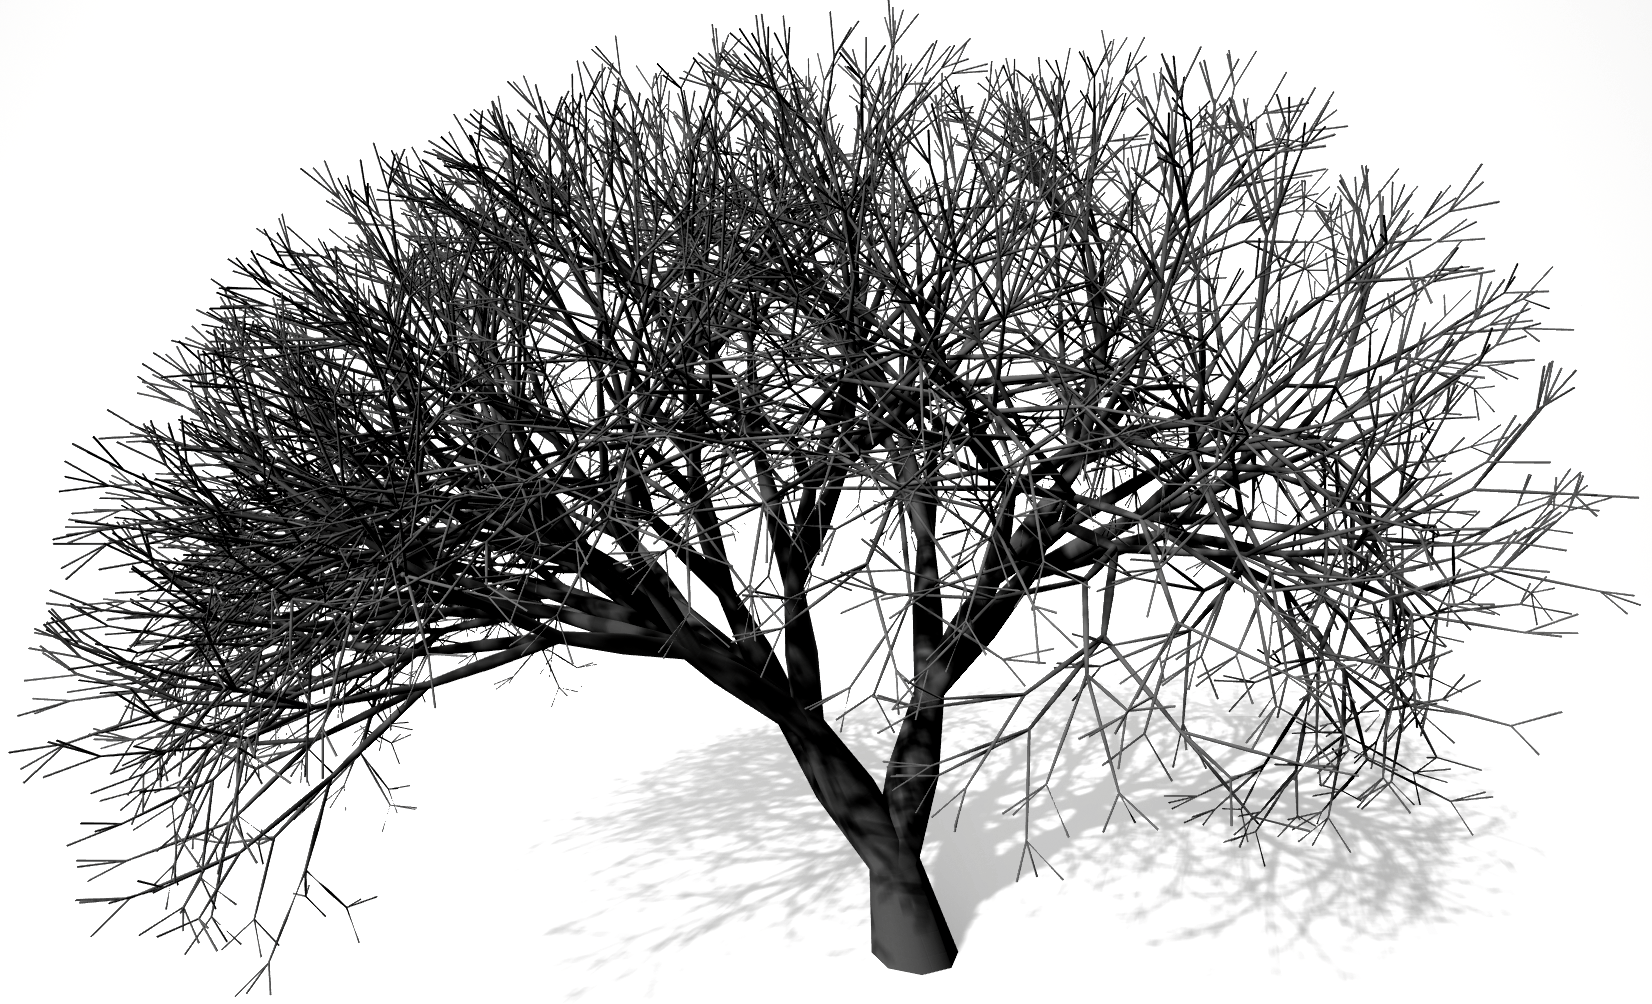
\includegraphics[height=.9\textheight]{images/Performance_LS_Ternary_4_Tropism}
	
	
	$\text{Generierungszeit}= 0.233s$, $206658 \text{ Vertizes}$
\end{center}




\newpage
\begin{center}
	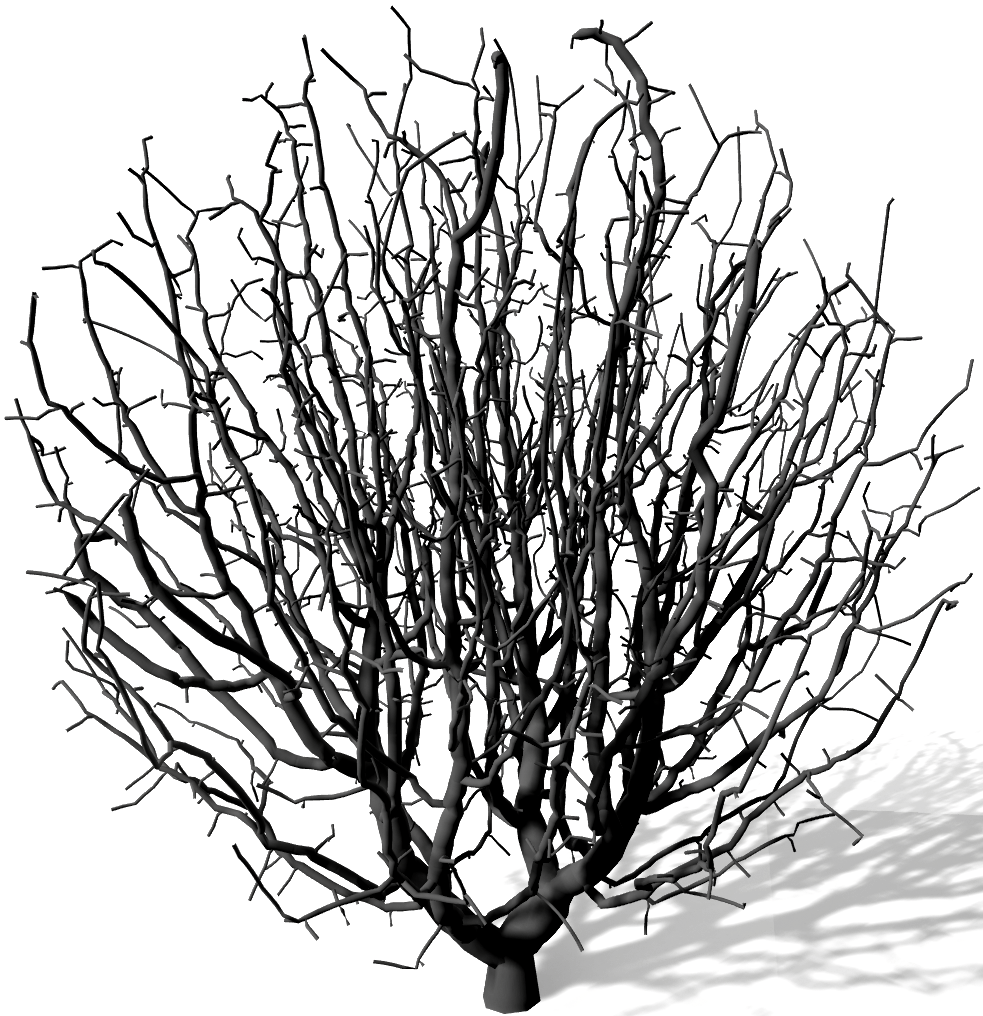
\includegraphics[height=.9\textheight]{images/Performance_SCA_Quali_Segments_High}
	
	$\text{Generierungszeit} = 2.416s$, $103725 \text{ Vertizes}$
\end{center}






\newpage
\subsection{Bewertung der Ergebnisse - Benutzerfreundlichkeit\\}

\paragraph{L-Systeme}
\begin{itemize}
	\item Verlangen vom Benutzer:
	\begin{itemize}
		\item Genaue Vorstellung der Baumstruktur
		\item Kenntnisse über L-System Definitionen
		\item Verständnis für die Umsetzung als L-System
	\end{itemize}
\end{itemize}


\paragraph{Space Colonization Algorithmus}
\begin{itemize}
	\item Klare Zusammenhänge zwischen Parametern und Baumstrukturform
	
	\item \glqq Trial and Error\grqq-Vorgehen möglich
\end{itemize}




\newpage
\slidetitle{6. Zusammenfassung - Erweiterungen}
\subsection{Wünschenswerte Erweiterungen\\}

\begin{itemize}
	\item Generierung zur Laufzeit\\
	
	\item Level-of-Detail (LOD)\\
	
	\item Oberflächenbeschaffenheit\\
	
	\item Blätter\\
	
	\item Verteilung der Baumstrukturen
\end{itemize}


\newpage
\begin{itemize}
	\item Space Colonization Algorithmus:
	\begin{itemize}
		\item Positionsabfragen\\
		
		\item Einflussbereiche\\
		
	\end{itemize}
\end{itemize}

\begin{itemize}
	\item L-Systeme:
	\begin{itemize}
		\item Erweiterungen\\
		
		\item Benutzerfreundlichkeit\\
		
		\item Einsatz vordefinierter Modelle
	\end{itemize}
\end{itemize}




\newpage
\slidetitle{7. Literatur}
\nocite{*}




